\chapter{Практическая часть}

\lstset{language=prolog}

\section{Создание проекта}
На рисунках \ref{img:general}, \ref{img:target}, \ref{img:warnings} изображен процесс создания проекта.
\begin{figure}[H]
    \centering
    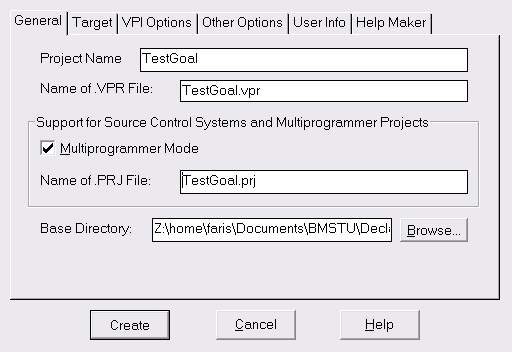
\includegraphics[scale=.7]{imgs/general.png}
    \caption{}
    \label{img:general}
\end{figure}
\begin{figure}[H]
    \centering
    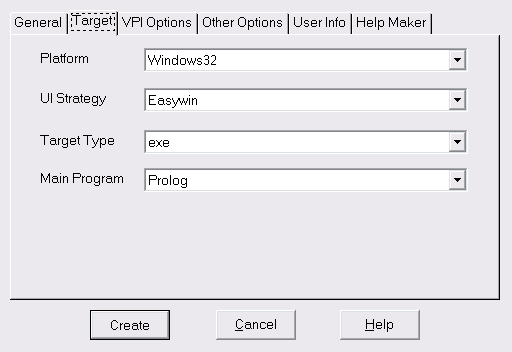
\includegraphics[scale=.7]{imgs/target.png}
    \caption{}
    \label{img:target}
\end{figure}
\begin{figure}[H]
    \centering
    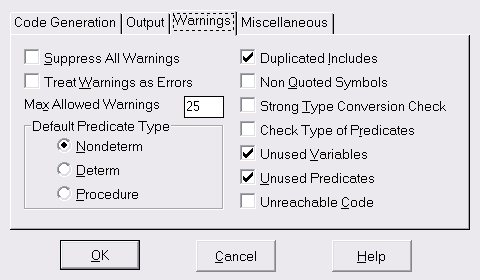
\includegraphics[scale=.7]{imgs/warnings.png}
    \caption{}
    \label{img:warnings}
\end{figure}

На рисунке \ref{img:first} приведен пример простой программы, подтверждающий работоспособность созданного проекта.
\begin{figure}[H]
    \centering
    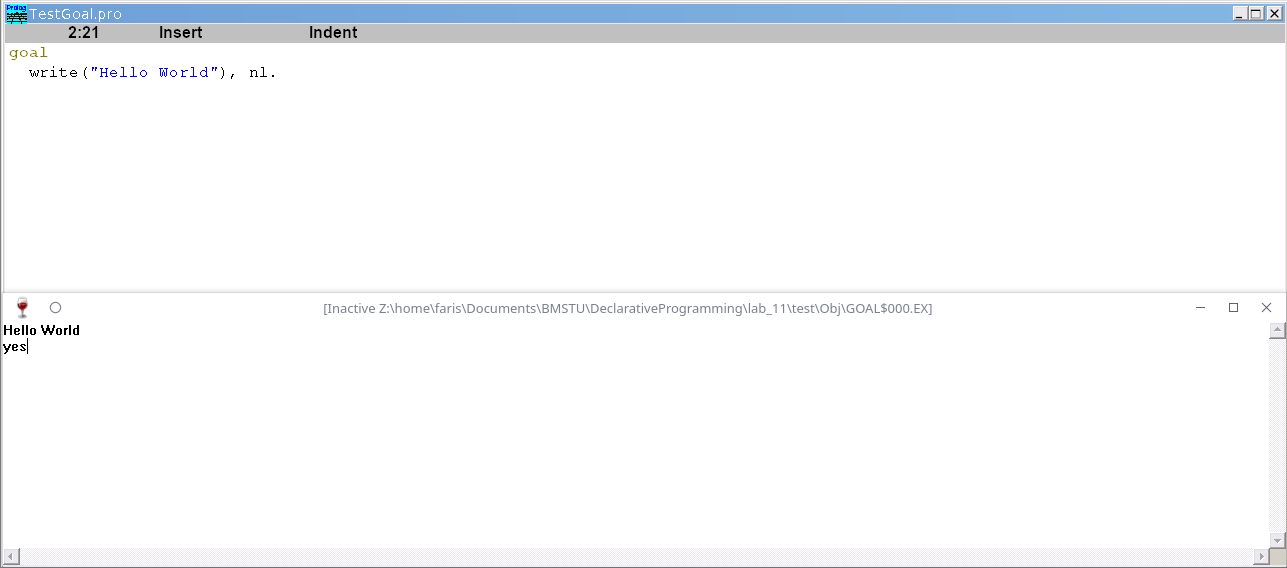
\includegraphics[scale=.5]{imgs/first.png}
    \caption{}
    \label{img:first}
\end{figure}

\section{Тестовая программа}
На рисунке \ref{img:test} приведен текст тестовой программы, результатом которой является ответ на вопрос ``Играет ли Билл в бейсбол?''.
\begin{figure}[H]
    \centering
    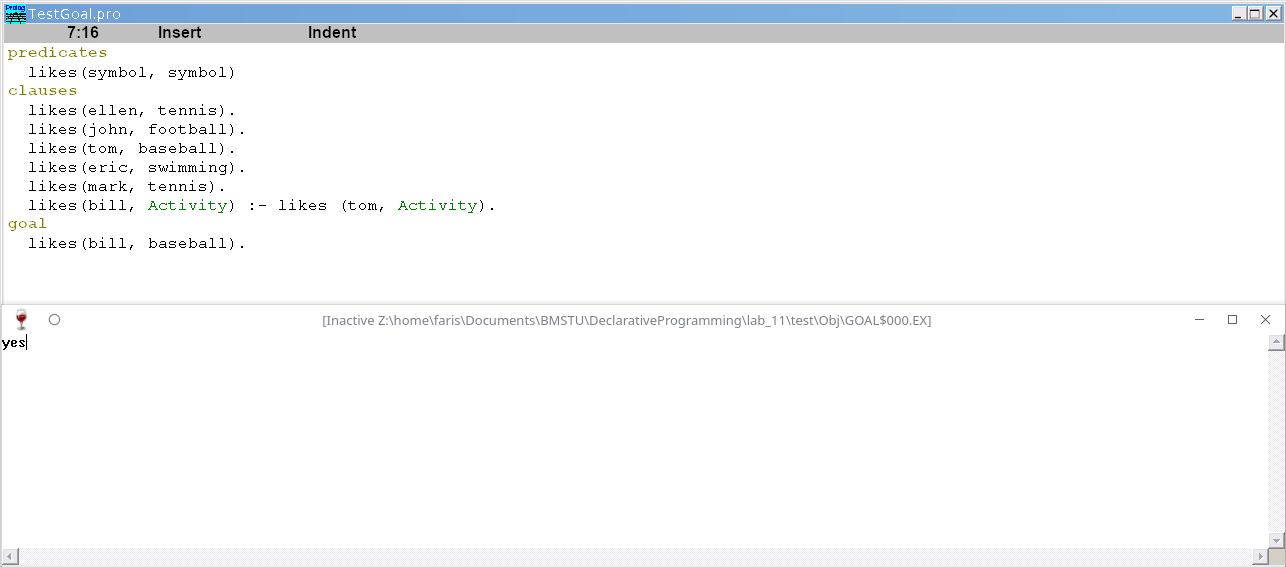
\includegraphics[scale=.5]{imgs/test.png}
    \caption{}
    \label{img:test}
\end{figure}
Такой результат объясняется тем, что база знаний данной программы содержит информацию о том, что, если Тому нравится некоторая активность, то она нравится Биллу. При этом Тому нравится бейсбол.

На рисунке \ref{img:solutions} приведен пример программы, результат который недетерминирован, то есть состоит из нескольких вариантов ответа на вопрос.
\begin{figure}[H]
    \centering
    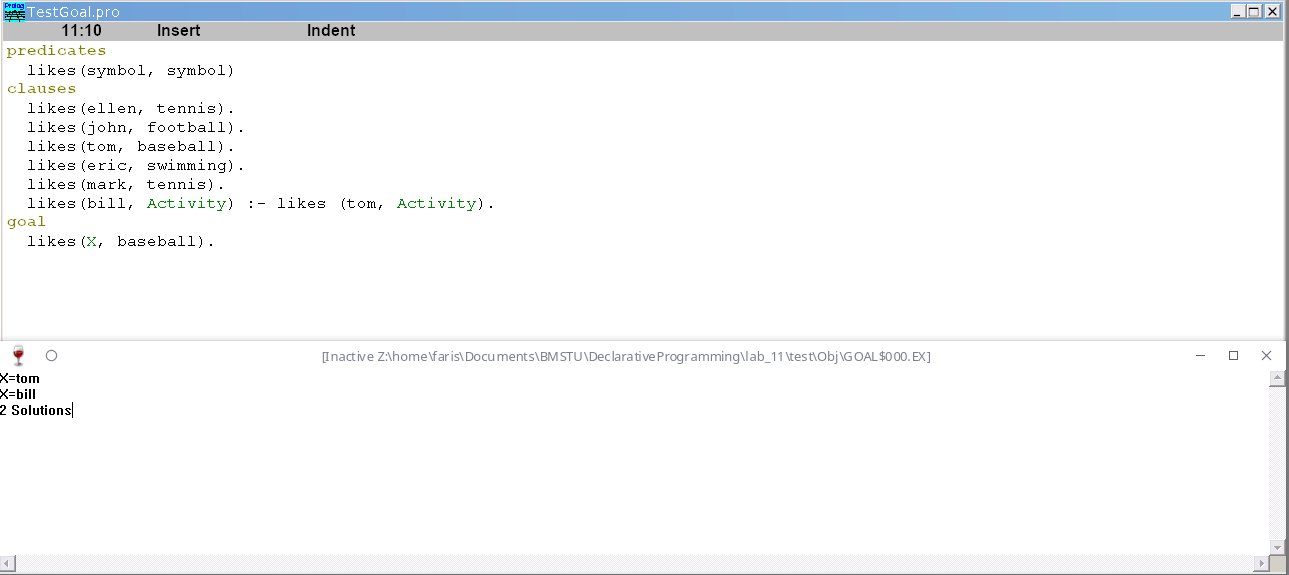
\includegraphics[scale=.5]{imgs/solutions.png}
    \caption{}
    \label{img:solutions}
\end{figure}

На рисунке \ref{img:debug} изображён режим отладки на примере тестовой программы.
\begin{figure}[H]
    \centering
    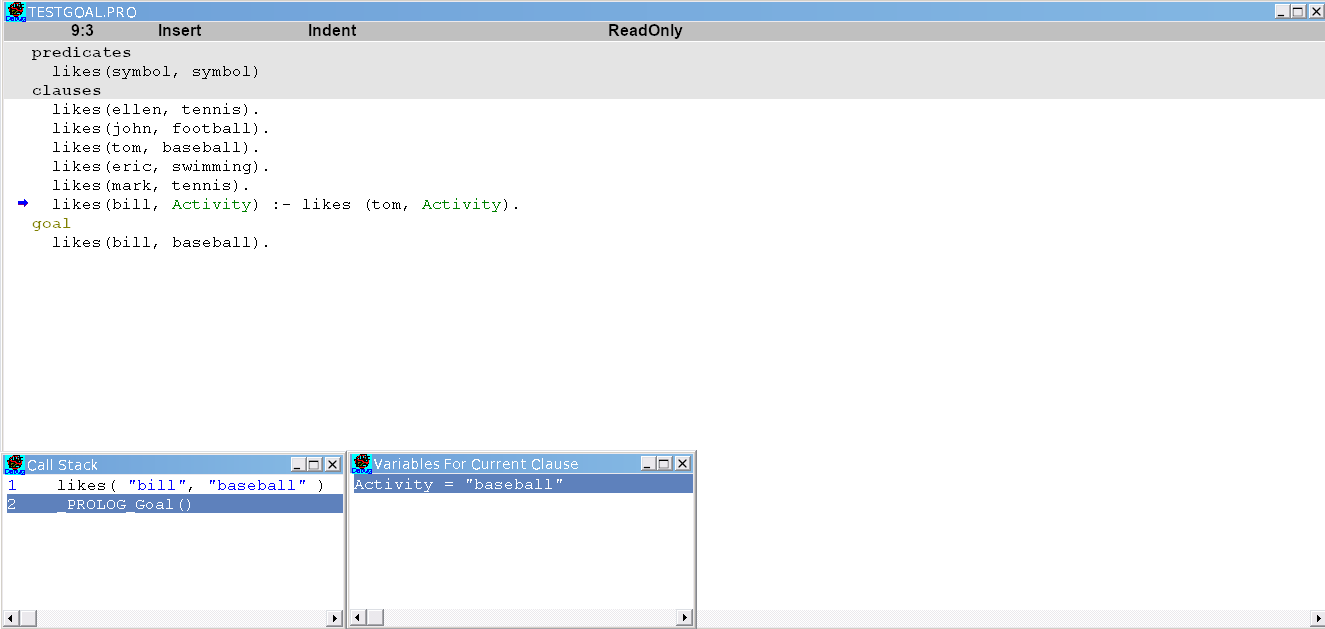
\includegraphics[scale=.45]{imgs/debug.png}
    \caption{}
    \label{img:debug}
\end{figure}

\section{Телефонный справочник}
Была разработана и успешно протестирована программа "Телефонный справочник". На рисунке \ref{img:phonebook1} изображен текст программы, содержащий вопрос о принадлежности номера \textbf{+7 314-82-53} человеку по имени \textbf{igor}, а на рисунке \ref{img:phonebook2} - какие номера в принципе ему принадлежат.
\begin{figure}[H]
    \centering
    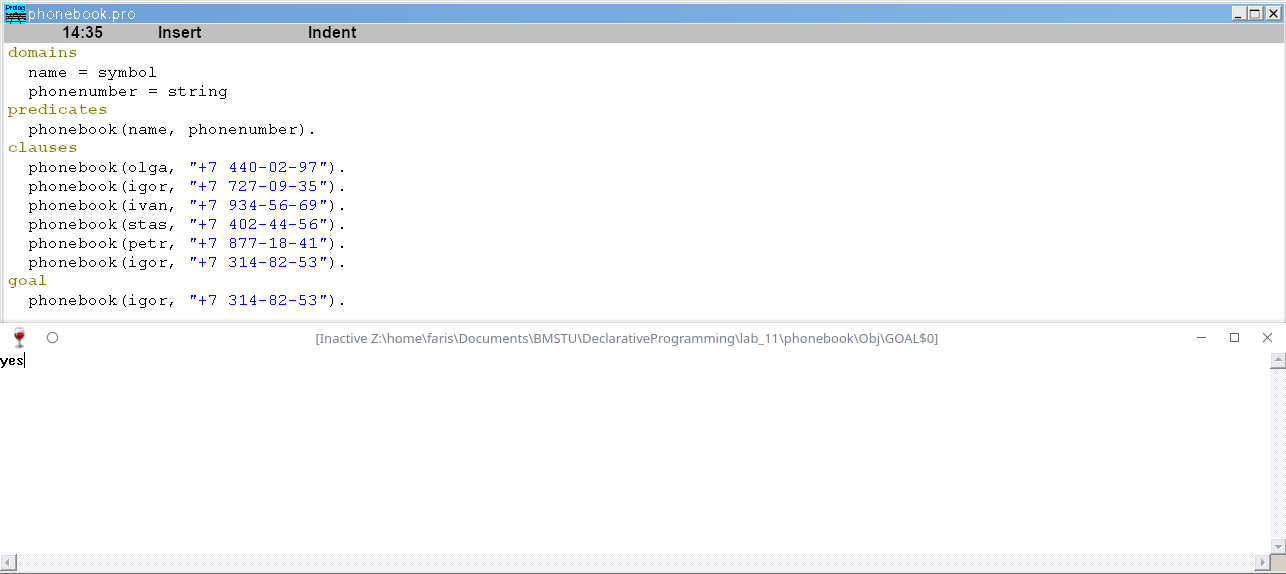
\includegraphics[scale=.5]{imgs/phonebook1.png}
    \caption{}
    \label{img:phonebook1}
\end{figure}
\begin{figure}[H]
    \centering
    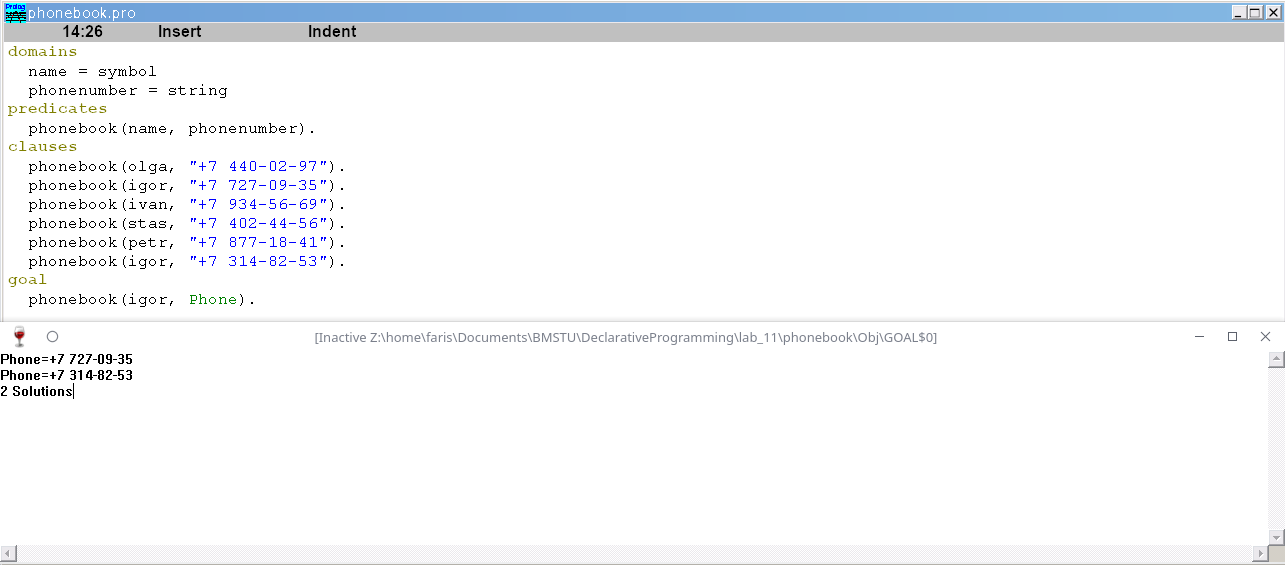
\includegraphics[scale=.5]{imgs/phonebook2.png}
    \caption{}
    \label{img:phonebook2}
\end{figure}

